\chapter{Grundlagen \& Stand der Technik}
\label{kap:Grundlagen}
\minitoc\pagebreak

\todo{mehr Quellen und ausgearbeiteter}

\section{Visualisierung von Daten}
\label{sec:visual}
Ein großer Aspekt dieser Arbeit ist das Darstellen und Visualisieren von gemessenen oder generierten Daten.
Dies beschreibt den Vorgang vorhandene Daten, die in heterogenen Formaten und Typen vorliegen, in eine visuelle, grafische Form umzuwandeln, sodass sie für den Menschen leichter wahrzunehmen und lesbar sind.
Mit einem einzigen Blick können mehrere Tausend Daten(-punkte) auf einmal verarbeitet werden.
Dabei kommt die Visualisierung zuerst als Sinnes-Reiz beim Betrachter an, daraufhin wird sie identifiziert, wahrgenommen und interpretiert \cite{Goldstein.2015, FischerStabel.2018}.
Für die gleiche Datenmenge bräuchte ein Mensch unvergleichbar mehr Zeit, um die selbige Interpretation der Daten zu erhalten.

Diese Möglichkeit, der schnellen und effizienten Interpretation für die vorliegenden Daten dieser Arbeit  bereitzustellen, ist eine der Zielstellungen.
Hierfür müssen vorab diverse Grundlagen gelegt werden, damit diese bei der späteren \fullref{kap:anforderungsanalyse}, \fullref{kap:konzept} und \fullref{kap:umsetzung} stets beachtet werden.

\subsection{Definitionen}
Zunächst werden grundlegende Begriffe wie Daten, Datenanalyse oder Visualisierung definiert, damit eine einheitliche Basis geschaffen wird.
\subsubsection{Daten}
Daten sind gemäß \cite{Dudenredaktion.2015}:
\begin{quote}
\glqq durch Beobachtungen, Messungen, statistische Erhebungen gewonnene [Zahlen]werte, [...] Angaben, formulierbare Befunde. \\
EDV: elektronisch gespeicherte Zeichen, Angaben, Informationen\grqq{}
\end{quote}

Demnach gibt es heterogene Daten, welche in Form von Zahlen, Buchstaben, Texten vorliegen können.
In Anblick auf die vorliegenden Daten dieser Arbeit gibt es beispielsweise gemessene Vitaldaten von Patienten wie Herz- \& Atemfrequenz oder die Sauerstoffsättigung.
Weiter sind auch vereinzelt Angaben zu dem Patienten, wie das Alter, oder generelle Informationen wie der Tag und die Uhrzeit eines Einsatzes als Daten gespeichert.
 
\subsubsection{Datenanalyse}
\label{subsub:datenanalyse}
Daten können analysiert werden.
Dabei bezeichnet die Analyse die strukturierte Untersuchung von Elementen, welche zunächst aufgeteilt und geordnet werden, damit anschließend eine Auswertung betrieben werden kann.
Dabei kann laut Fischer \cite{Fischer.2014} grundlegend zwischen zwei Formen der Analyse unterschieden werden: konfirmativ und explorativ.
\begin{description}
\item[konfirmative Analyse] bezeichnet die Überprüfung von bestehenden Hypothesen.
Dabei werden bekannte Methoden angewandt, um die jeweilige Hypothese zu bestätigen oder zu widerlegen.
\item[explorative Analyse] ist gekennzeichnet durch das Fehlen von gestellten Hypothesen.
Hierbei wird nach neuen Erkenntnissen oder Fragestellungen gesucht, welche durch Trends, Muster oder Beziehungen entdeckt werden.
\end{description}

Da bei dieser Arbeit das zu untersuchende Element der Analyse stets Daten sind, handelt es sich in diesem Kontext immer um \glqq Datenanalysen\grqq{} \cite{Schumann.2000}.
Es kommen hier sowohl explorative als auch konfirmative Datenanalysen zum Einsatz, da es bereits bestehende Hypothesen in Form von Fragestellungen der Nutzer gibt.
Andererseits gibt es auch vermeintlich viele, bisher unbekannte, Zusammenhänge, welche durch die Interaktion der Anwender mit den Visualisierungen zum Vorschein kommen können.


\subsubsection{Visualisierung}
\label{subsub:visual}
Eine Visualisierung ist nach McCormick \cite{Mccormick.1987} das transformation von Information in geometrische Repräsentation von graphischen Objekten.
Dies erleichtert dem Menschen die Aufnahme von Informationen, insbesondere aber das erkennen von Zusammenhängen und Strukturen innerhalb der Daten.
Die Subjektivität der Individuen ermöglicht keine einwandfreie Garantie des Informationsflusses zum jeweiligen Anwender. %\cite{Fischer.2014}. 
Auch kann unterschieden werden, ob eine Visualisierung unterstützend zu einer Niederschrift beiträgt, oder sie als Haupt-Informationsquelle die tragende Figur ist \cite{Bassler.2010}.
Im Zuge dieser Arbeit wird letzteres das Mittel der Wahl sein.

Nach \cite{Card.2007} kann die Datenvisualisierung als besondere Form einer Visualisierung abgegrenzt werden.
Dabei gibt es fünf Eigenschaften, die eine solche spezielle Form klassifizieren:
\begin{itemize}
\item Computergestützte Anzeige 
\item Der Nutzer kann interaktiv Auswahlen treffen oder Filter bestimmen, um die anzuzeigenden Daten einzuschränken
\item Die Eigenschaften der Daten werden in visuellen Elementen wie Form, Farbe oder Größe unterschiedlich dargestellt
\item Abstrakte Daten können dargestellt werden, welche keiner physischen Form zugrunde liegen
\item Die Fähigkeiten des Menschen in Bezug auf die Wahrnehmung wird berücksichtigt 
\end{itemize}

Demzufolge wird im Kontext dieser Arbeit der Begriff Datenvisualisierung und Visualisierung synonym verwendet, da die entsprechenden Eigenschaften auf die hier erarbeiteten Visualisierungen zutreffen.
%\todotext{konfirmativ und explorativ visualis (fischer s.26?}

%WordCloud
Es gibt nach \cite{Schumann.2000} einen \glqq Visualisierungsprozess\grqq{}, welcher den Weg von Rohdaten bis zum Bild abstrahieren soll.

\bild
{visualprozess}
{8cm}
{Der Prozess einer Visualisierung von den Rohdaten zum fertig generierten Bild. Bildquelle \cite[S.50]{FischerStabel.2018} (verändert)}
{Der Prozess einer Visualisierung}

Dieser Prozess ist in Abbildung \ref{fig:visualprozess} erkennbar.
Nachfolgend werden die einzelnen Phasen kurz erläutert:
\begin{description}
\item[Rohdaten] In der ersten Phase muss eine oder mehrere Quellen der Daten festgelegt werden. 
Anschließend wird grob gesichtet und so eine Datenbasis gelegt.
\item[Filtering] Anschließend werden die Rohdaten aufbereitet, wobei beispielsweise eine Bereinigung, Interpolation oder Neuberechnung von Daten vorgenommen werden
\item[Mapping] Daraufhin kommt nach \cite{FischerStabel.2018} das Hauptproblem der Visualisierung: Die Auswahl einer geeignet Darstellungsform passend zu den Daten. 
Dabei gibt es diverse Möglichkeiten, welche Darstellungsform mit welchen Attributen (Größe, Farbe, Form) umgesetzt wird. 
\item[Rendering] Als Letztes werden die aufbereiteten Daten mit der gewählten Darstellungsform als Bild oder interaktive Visualisierung erzeugt.
Dies geschieht heutzutage häufig über sogenannte \gls{BI}-Werkzeuge wie Qlik (siehe \ref{sub:qlik})
\end{description}




\subsection{Gestaltungsgrundsätze}
\label{sub:grundsaetze}
In der Wahrnehmungspsychologie gibt es diverse Erkenntnisse, wie das menschliche Gehirn unterschiedliche Muster und Strukturen erkennt.
Dabei sind diese Fähigkeiten größtenteils evolutionär geprägt, da es für den Menschen schon immer wichtig war, schnell Entscheidungen zu treffen, oder komplexe neue Aufgabestellungen zu lösen.
Dabei greift das Gehirn auf zuvor erlernten oder erlebten Ereignissen zurück, um neue Aufgaben klassifizieren zu können.

Heutzutage finden sich die Auswirkungen dieser Prägungen in dem Alltag jedes Menschen wieder.
Dabei ist die Form der Wahrnehmung nie objektiv, sondern stets subjektiv, da diese Fähigkeit der Mustererkennung auf Basis von Erfahrungen aufbaut, welche bei jedem Menschen im Laufe des Lebens unterschiedlich sind.
Dies ist eine wichtige und essentielle Erkenntnis, da hierbei die Interpretation von Datenvisualisierungen divergieren kann \cite{Fischer.2014}.

Dennoch gibt es diverse Grundregeln, welche sich im Laufe der Jahrtausende bei den Menschen durchgesetzt haben. Diese wurden zuerst von Wertheim in seiner Forschung \glqq Lehre von der Gestaltung\grqq{} schriftlich festgehalten \cite{Wertheimer.2017}.
Nach und nach wurden diese von mehreren Psychologen oder Designern unter den \glqq Gestaltungs-Gesetzen\grqq{} oder -Prinzipien aufgefasst undabgewandelt, wodurch sie sich indes unterscheiden.
Nachfolgend werden fünf, für Diagramme und Visualisierungen relevante Gesetze nach \cite[5.2]{Heber.2018} \& \cite{Ware.2009} näher betrachtet. 
Hierbei sind vor allem bei Visualisierungen mit Zahlen, wie sie in dieser Arbeit größtenteils vorliegen werden, die ersten beiden Gesetze von sehr hoher Relevanz.

\subsubsection{Das Gesetz der Nähe}
\begin{figure}[ht]
\begin{subfigure}{.5\linewidth}
  \centering
  % include first image
  
\includegraphics[width=.95\linewidth]{img/gNaehe}  
  \caption{Schematische Darstellung zur Nähe}
  \label{fig:naeheSchema}
\end{subfigure}
\begin{subfigure}{.5\linewidth}
  \centering
  % include second image
  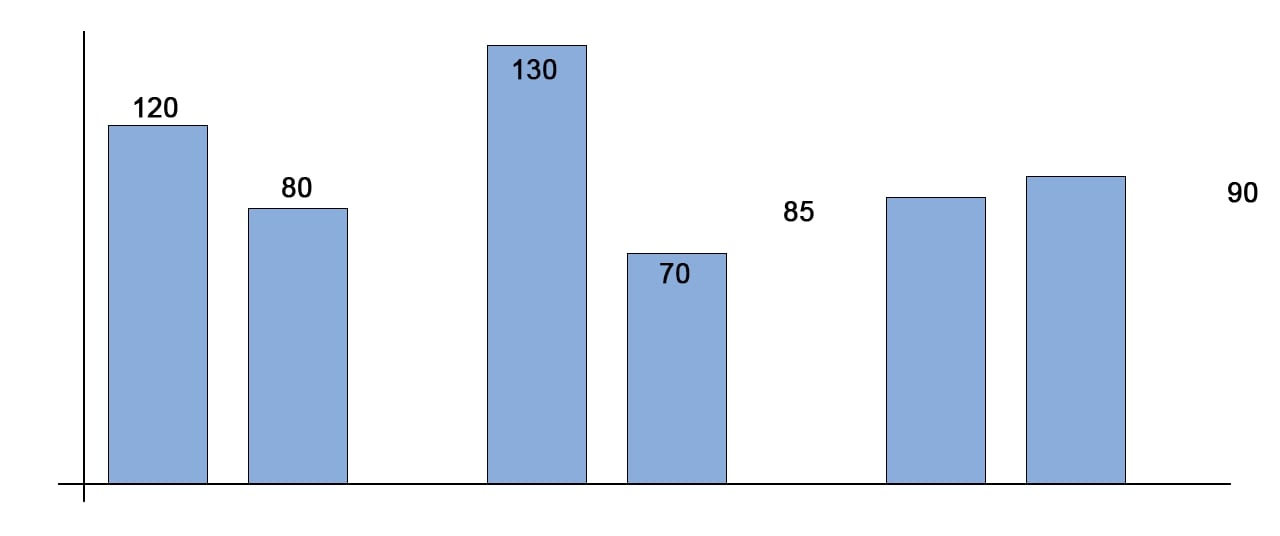
\includegraphics[width=.95\linewidth]{img/gNaeheDia}  
  \caption{Beispiel an einem Balkendiagramm mit zwei positiven und einem negativen (rechts) Beispiel}
  \label{fig:naeheDia}
\end{subfigure}
\caption[Gesetz der Nähe]{Eigene Darstellung des Gesetzes der Nähe. Links schematisch und rechts an einem Balkendiagramm dargestellt}
\label{fig:naehe}
\end{figure}
%\bild
%{gNaehe}
%{8cm}
%{Beispiel des Gesetzes der Nähe. Eigene Darstellung}
%{Gesetz der Nähe}

Das Gesetz der Nähe besagt, dass Elemente, die nahe beieinander liegen, als eine Einheit wahrgenommen werden.
Dieser Effekt ist in Abbildung \ref{fig:naehe} veranschaulicht.
Für Visualisierungen und insbesondere Diagramme bedeutet dies, dass sich beispielsweise die Zahlen immer in der Nähe des entsprechenden Elements befinden sollten.

In \ref{fig:naeheDia} ist dieser Effekt deutlich zu erkennen. 
Zum einen werden immer zwei Balken aufgrund der Distanz als Zusammengehörig wahrgenommen, zum anderen sind die Zahlen bei den ersten vier Balken gut zuzuordnen.
Bei den letzten zwei Balken sind die Zahlen zu weit entfernt und können den jeweiligen Betrachter verwirren.


\subsubsection{Das Gesetz der Ähnlichkeit}
\label{subsub:ähnlich}
\begin{figure}[ht]
\begin{subfigure}{.5\linewidth}
  \centering
  % include first image
  
\includegraphics[width=.95\linewidth]{img/gAehnlich}  
  \caption{Schematische Darstellung zur Ähnlichkeit}
  \label{fig:aehnlichSchema}
\end{subfigure}
\begin{subfigure}{.5\linewidth}
  \centering
  % include second image
  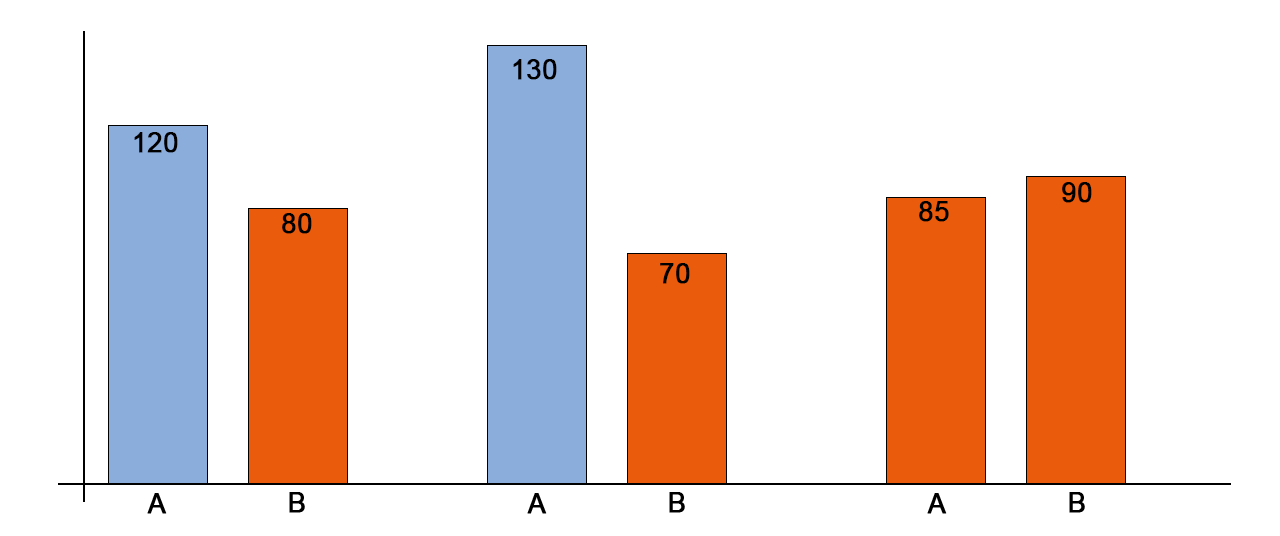
\includegraphics[width=.95\linewidth]{img/gAehnlichDia}  
  \caption{Beispiel an einem Balkendiagramm mit zwei positiven und einem negativen (rechts) Beispiel}
  \label{fig:aehnlichDia}
\end{subfigure}
\caption[Gesetz der Ähnlichkeit]{Eigene Darstellung des Gesetzes der Ähnlichkeit. Links schematisch und rechts an einem Balkendiagramm dargestellt}
\label{fig:aehnlich}
\end{figure}

Ebenfalls als eine Gruppe werden Elemente wahrgenommen, die ähnlich oder gleich aussehen.
Dabei spielen unterschiedliche Attribute wie Größe, Form oder Farbe eine Rolle.
Hier gilt, je mehr Ähnlichkeit die Elemente besitzen, desto stärker wirken sie als Einheit.

An einem Balkendiagramm ist dieses Gesetz in \ref{fig:aehnlichDia} dargestellt.
Die blauen und orangefarbenen Balken werden als Teile einer Gruppe wahrgenommen.
Die letzten beiden Balken verdeutlichen wieder ein Negativ-Beispiel: Hier werden die Balken fälschlicherweise einer Gruppe zugeordnet, obwohl sie zu zwei unterschiedlichen Gruppen gehören.
Hier wirkt außerdem das Gesetz der Nähe.


\subsubsection{Das Gesetz der Geschlossenheit}
\bild
{gGeschlossenheit}
{8cm}
{Beispiel des Gesetzes der Geschlossenheit. Eigene Darstellung}
{Gesetz der Geschlossenheit}

Das Gesetz der Geschlossenheit besagt, dass Strukturen und Formen notorisch vervollständigt werden.
Außerdem werden die vervollständigten Formen als eine zusammengehörige Gruppe wahrgenommen.

\subsubsection{Das Gesetz der Erfahrung}
\begin{figure}[ht]
\begin{subfigure}{.5\linewidth}
  \centering
  % include first image
  
\includegraphics[width=.95\linewidth]{img/gErfahrung}  
  \caption{Vervollständigung des Wortes \glqq Erfahrung\grqq}
  \label{fig:erfahrung1}
\end{subfigure}
\begin{subfigure}{.5\linewidth}
  \centering
  % include second image
  
\includegraphics[width=.95\linewidth]{img/gErfahrung2}  
  \caption{Ein minimalistisches (links) und ein detailliertes Haus. Beide sind sofort zu erkennen}
  \label{fig:erfahrung2}
\end{subfigure}
\caption[Gesetz der Erfahrung]{Eigene Darstellung des Gesetzes der Erfahrung}
\label{fig:erfahrung}
\end{figure}
Das Gesetz der Erfahrung, oftmals auch der Einfachheit oder guten Gestalt genannt, bewirkt, dass unbekannte Objekte stets mit bereits bekannten Objekten abstrahiert werden.
Auch können verdeckte Texte wie in \ref{fig:erfahrung1} trotz fehlender teile gelesen werden.
Doch wenn zu viel Information verdeckt ist, ist auch keine Abstraktion auf bekannte Objekte möglich.

Bei \ref{fig:erfahrung2} wird deutlich, dass mit minimalen Informationen das Objekt klar wird.
Es sind keine Fenster, Türen, Schornstein oder anderes notwendig, damit das linke Objekt als Haus erkannt wird.

%Einfachheit
%der guten Gestalt}
\subsubsection{Das Gesetz der guten Fortsetzung}
\begin{figure}[ht]
\begin{subfigure}{.5\linewidth}
  \centering
  % include first image
  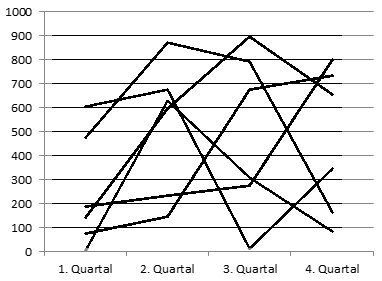
\includegraphics[width=.95\linewidth]{img/gFort}  
  \caption{Ein Liniendiagramm mit vielen schwarzen Linien}
  \label{fig:fort1}
\end{subfigure}
\begin{subfigure}{.5\linewidth}
  \centering
  % include second image
  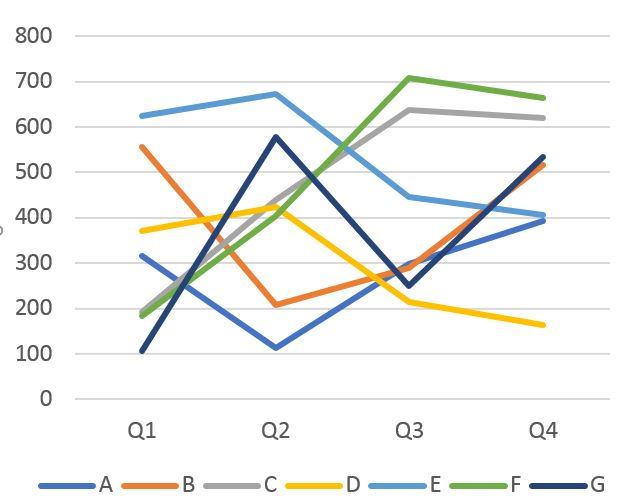
\includegraphics[width=.95\linewidth]{img/gFortC}  
  \caption{Verbesserte Lesbarkeit durch zusätzliches berücksichtigen des Gesetztes der Ähnlichkeit}
  \label{fig:fort2}
\end{subfigure}
\caption[Gesetz der Fortsetzung]{Darstellung des Gesetzes der guten Fortsetzung}
\label{fig:fort}
\end{figure}

Durch das Gesetz der guten oder stetigen Fortsetzung nehmen Menschen beispielsweise kreuzende Formen so wahr, wie sie für uns am einfachsten fortgesetzt werden.
Dies ist insbesondere bei Liniendiagrammen der Fall.

In Abbildung \ref{fig:fort1} sind trotz der vielen gleichfarbigen Linien die Verläufe der einzelnen Kurven dank dieses Prinzips gut erkennbar.
Um jedoch in späteren Anwendungen die Nutzerfreundlichkeit zu erhöhen und Komplexität zu mindern, kann in einem solchen Fall das Gesetz der Ähnlichkeit (siehe \ref{subsub:ähnlich}) zusätzlich angewandt werden.
Die bessere Lesbarkeit ist in \ref{fig:fort2} zu erkennen.

\subsection{Statistische Auswertungen}
\subsubsection{Definition Diagramme}
Wie im zuvor bearbeiteten Kapitel zu sehen ist, wurden als Veranschaulichung der Gestaltungsgrundsätze bereits Diagramme verwendet.
Ein Diagramm ist \glqq eine grafische Darstellung von Größenverhältnissen beziehungsweise Zahlenwerten in anschaulicher, leicht überblickbarer Form\grqq{} (Vgl. \cite{Dudenredaktion.2015}).
Wie in \ref{subsub:visual} bereits untersucht, sind Datenvisualisierungen eine besondere Form von Visualisierungen.
Diagramme sind wiederum eine besondere Form der Datenvisualisierungen, da sie die fünf Eigenschaften nach \cite{Card.2007} erfüllen, welche eine Datenvisualisierung klassifizieren (siehe S. \pageref{subsub:visual}). 

\subsubsection{(Verschiedene) Arten von Diagrammen und deren Nutzen}
Es gibt dabei eine Vielzahl von Diagrammkategorien, die weit über die klassischen Balken- oder Liniendiagramme hinaus gehen.
Darunter fallen Hyperonyme wie Achsendiagramme, Flussdiagramme (Organigramme), Zeitstrahl, Relationsdiagramme oder spezielle Diagramme in besonderen Fachrichtungen wie ein Klassen(UML)-Diagramm in der Informatik oder ein Grotrian-Diagramm in der Physik \cite{Duncan.2018, Bounford.2001, Engels.2015}.

Im Rahmen dieser Arbeit werden größtenteils die klassischen Achsendiagramme und ein paar spezielle Diagramme beleuchtet.
Dies hängt mit der Intention, der Technologie und den vorliegenden Daten zusammen, da hierfür Kennzahlen und Dimensionen mit- und untereinander in Beziehungen gebracht werden, um neue Erkenntnisse zu erlangen oder Hypothesen zu bearbeiten.

Ein Beispiel dafür, wie effektiv die kognitive Erleichterung durch die grafische Präsentation von Zahlenwerten funktioniert, zeigt das folgende Beispiel:

\begin{table}[htb]
\centering
%\resizebox{\textwidth}{!}{%
\begin{tabular}{|l|l|l|l|}
\hline
\textbf{Kunde}                  & \textbf{Umsatz} & \textbf{Gewinn} & \textbf{Umsatzmarge} \\ \hline
Acer                               & 9.342.856      & 3.513.673             & 37,6\%                     \\ \hline
Boston and Albany Railroad Company & 5.581.529      & 1.924.006             & 34,5\%                     \\ \hline
Calypso                            & 2.327.940      & 1.258.510             & 54,1\%                     \\ \hline
Champion International             & 1.972.009      & 835.208               & 42,4\%                     \\ \hline
Edna Design                        & 2.044.386      & 900.829               & 44,1\%                     \\ \hline
Fokas                              & 1.934.520      & 829.052               & 42,9\%                     \\ \hline
Information Bureau                 & 2.419.778      & 1.097.471             & 45,4\%                     \\ \hline
%J. S. Lee Associates               & 2.048.522      & 263.119               & 12,8\%                     \\ \hline
%KENROB and Associates              & 3.691.399      & 1.671.433             & 45,3\%                     \\ \hline
%Matradi                            & 3.108.910      & 903.906               & 29,1\%                     \\ \hline
%Pacifico                           & 2.248.193      & 464.785               & 20,7\%                     \\ \hline
%Paracel                            & 11.117.286     & 5.077.890             & 45,7\%                     \\ \hline
%Renegade info Crew                 & 1.782.516      & 870.276               & 48,8\%                     \\ \hline
Road Warrior International         & 3.127.719      & 948.304               & 30,3\%                     \\ \hline
Talarian                           & 9.168.719      & 3.281.944             & 35,8\%                     \\ \hline
Tandy Corporation                  & 11.889.136     & 5.585.705             & 47,0\%                     \\ \hline
Target                             & 5.369.579      & 1.711.586             & 31,9\%                     \\ \hline
Teammax                            & 2.009.436      & 1.055.986             & 52,6\%                     \\ \hline
Unison Management Concepts         & 2.115.465      & 1.083.508             & 51,2\%                     \\ \hline
Vanstar                            & 3.720.451      & 1.616.382             & 43,4\%                     \\ \hline
\end{tabular}%
%}
\caption[Beispiel einer Datentabelle]{Ein Beispiel einer Datentabelle mit vier Spalten, mehreren Zeilen und diversen Werten}
\label{tbl:data}
\end{table}


%booktabs table
%\begin{table}[]
%\centering
%\resizebox{\textwidth}{!}{%
%\begin{tabular}{@{}llll@{}}
%\toprule
%\textbf{Customer}                                        & \textbf{Sales}                  & \textbf{Sales Margin}          & \textbf{Sales Margin (\%)}  \\ \midrule
%\multicolumn{1}{|l|}{Acer}                               & \multicolumn{1}{l|}{9.342.856}  & \multicolumn{1}{l|}{3.513.673} & \multicolumn{1}{l|}{37,6\%} \\ \midrule
%\multicolumn{1}{|l|}{Boston and Albany Railroad Company} & \multicolumn{1}{l|}{5.581.529}  & \multicolumn{1}{l|}{1.924.006} & \multicolumn{1}{l|}{34,5\%} \\ \midrule
%\multicolumn{1}{|l|}{Calypso}                            & \multicolumn{1}{l|}{2.327.940}  & \multicolumn{1}{l|}{1.258.510} & \multicolumn{1}{l|}{54,1\%} \\ \midrule
%\multicolumn{1}{|l|}{Champion International}             & \multicolumn{1}{l|}{1.972.009}  & \multicolumn{1}{l|}{835.208}   & \multicolumn{1}{l|}{42,4\%} \\ \midrule
%\multicolumn{1}{|l|}{Edna Design}                        & \multicolumn{1}{l|}{2.044.386}  & \multicolumn{1}{l|}{900.829}   & \multicolumn{1}{l|}{44,1\%} \\ \midrule
%\multicolumn{1}{|l|}{Fokas}                              & \multicolumn{1}{l|}{1.934.520}  & \multicolumn{1}{l|}{829.052}   & \multicolumn{1}{l|}{42,9\%} \\ \midrule
%\multicolumn{1}{|l|}{Information Bureau}                 & \multicolumn{1}{l|}{2.419.778}  & \multicolumn{1}{l|}{1.097.471} & \multicolumn{1}{l|}{45,4\%} \\ \midrule
%\multicolumn{1}{|l|}{J. S. Lee Associates}               & \multicolumn{1}{l|}{2.048.522}  & \multicolumn{1}{l|}{263.119}   & \multicolumn{1}{l|}{12,8\%} \\ \midrule
%\multicolumn{1}{|l|}{KENROB and Associates}              & \multicolumn{1}{l|}{3.691.399}  & \multicolumn{1}{l|}{1.671.433} & \multicolumn{1}{l|}{45,3\%} \\ \midrule
%\multicolumn{1}{|l|}{Matradi}                            & \multicolumn{1}{l|}{3.108.910}  & \multicolumn{1}{l|}{903.906}   & \multicolumn{1}{l|}{29,1\%} \\ \midrule
%\multicolumn{1}{|l|}{Pacifico}                           & \multicolumn{1}{l|}{2.248.193}  & \multicolumn{1}{l|}{464.785}   & \multicolumn{1}{l|}{20,7\%} \\ \midrule
%\multicolumn{1}{|l|}{Paracel}                            & \multicolumn{1}{l|}{11.117.286} & \multicolumn{1}{l|}{5.077.890} & \multicolumn{1}{l|}{45,7\%} \\ \midrule
%\multicolumn{1}{|l|}{Renegade info Crew}                 & \multicolumn{1}{l|}{1.782.516}  & \multicolumn{1}{l|}{870.276}   & \multicolumn{1}{l|}{48,8\%} \\ \midrule
%\multicolumn{1}{|l|}{Road Warrior International}         & \multicolumn{1}{l|}{3.127.719}  & \multicolumn{1}{l|}{948.304}   & \multicolumn{1}{l|}{30,3\%} \\ \midrule
%\multicolumn{1}{|l|}{Talarian}                           & \multicolumn{1}{l|}{9.168.719}  & \multicolumn{1}{l|}{3.281.944} & \multicolumn{1}{l|}{35,8\%} \\ \midrule
%\multicolumn{1}{|l|}{Tandy Corporation}                  & \multicolumn{1}{l|}{11.889.136} & \multicolumn{1}{l|}{5.585.705} & \multicolumn{1}{l|}{47,0\%} \\ \midrule
%\multicolumn{1}{|l|}{Target}                             & \multicolumn{1}{l|}{5.369.579}  & \multicolumn{1}{l|}{1.711.586} & \multicolumn{1}{l|}{31,9\%} \\ \midrule
%\multicolumn{1}{|l|}{Teammax}                            & \multicolumn{1}{l|}{2.009.436}  & \multicolumn{1}{l|}{1.055.986} & \multicolumn{1}{l|}{52,6\%} \\ \midrule
%\multicolumn{1}{|l|}{Unison Management Concepts}         & \multicolumn{1}{l|}{2.115.465}  & \multicolumn{1}{l|}{1.083.508} & \multicolumn{1}{l|}{51,2\%} \\ \midrule
%Vanstar                                                  & 3.720.451                       & 1.616.382                      & 43,4\%                      \\ \bottomrule
%\end{tabular}%
%}
%\caption{My caption}
%\label{my-label}
%\end{table}

In Tabelle \ref{tbl:data} sind diverse Zahlen zu Kunden und deren Umsätze, Gewinn und Marge zu sehen.
Dabei ist die Informationsflut und daraus resultierende Reizüberflutung für den jeweiligen Betrachter ein Hindernis, um schnell neue Erkenntnisse zu gewinnen oder Vergleiche zu vollziehen.
Welcher Kunde beispielsweise den höchsten oder niedrigsten Umsatz, Gewinn oder Marge hat, ist in dieser Tabelle nicht sofort ersichtlich.

\bildbreit
{MuchDataBetter}
{Die Daten aus Tabelle \ref{tbl:data} in grafischer Form eines Kombinations-Diagrammes dargestellt}
{Daten aus Tabelle \ref{tbl:data} in grafischer Form eines Diagrammes dargestellt}

Eine deutliche Verbesserung der Interpretationsmöglichkeiten ist in Abbildung \ref{fig:MuchDataBetter} zu erkennen.
Hier sind die Daten aus Tabelle \ref{tbl:data} in visueller Form eines dargestellt.
Dabei ist das gewählte Diagramm eine Kombination aus Balken- und Liniendiagramm.

Es ist sofort möglich, den Kunden mit dem meisten und geringsten Umsatz ausfindig zu machen.
Gleichzeitig wird eine Relation des Unterschiedes sichtbar, da die Balkenhöhe gut miteinander verglichen werden kann.
Des Weiteren sind die Zahlen des Gewinnes und der Umsatzmarge als farbig unterscheidbare Striche in den Balken integriert.
Hierdurch sind weitere Beziehung sichtbar, welcher Kunde den höchsten oder niedrigsten Gewinn oder Umsatzmarge generiert.
Auch ist mühelos ein Zusammenhang zwischen Umsatz, Gewinn und Umsatzmarge jedes einzelnen Kunden ersichtlich, welcher wiederum sofort mit anderen Kunden verglichen werden kann.

Die Liste der schnell und effizient identifizierten neuen Erkenntnisse kann noch weiter geführt werden.
Als Motivation und Argument für die grafische Darstellung von solchen Zahlenwerten soll dieser Auszug jedoch genügen.

Eine kurze Auswahl an häufig relevanten Diagrammen und Visualisierungen wird im folgenden kurz erläutert:
\begin{description}
\item[Liniendiagramm] Ein Liniendiagramm ist eine nützliche Visualisierung, um zeitliche Verläufe darzustellen. 
Wenn also temporäre Daten aufgezeigt werden, die eine Veränderung zum nächsten Zeitpunkt aufweisen, kann die Verbindung der Datenpunkte durch Linien eine Abweichung grafisch untermauern. 
Ein Beispiel eines Liniendiagrammes ist in Abbildinug \ref{fig:fort2} zu erkennen.

\item[Balkendiagramm] Balkendiagramme zeigen die absoluten Werte von Daten an und visualisieren eine mögliche Differenz zu andern Balken \cite[S.54]{Bounford.2001}.
Die Balken gehen dabei üblicherweise von eine gemeinsamen Grundlinie aus, was sie von einem Liniendiagramm unterscheidet.
Dadurch können sehr kleine Änderungen bei großen absoluten Werten unter Umständen untergehen, was bei einem Liniendiagramm nicht der Fall ist, da diese keine Grundlinie bei 0 haben, sondern eine dynamische Y-Achsen-Skalierung nutzen können.

\bild
{kombi}
{14cm}
{Beispiel eines Kombinationsdiagramm aus Balken und einer Linie}
{Kombinationsdiagramm aus Balken und einer Linie}

In einem Kombinationsdiagramm werden in der Regel Balken und Linien oder Symbole miteinander kombiniert, um die Vorteile beider Typen in Anspruch zu nehmen.
Hierbei wird in der Regel eine sekundäre Y-Achse an der rechten Seite eines Diagrammes angelegt, welche die Skalierung für die Linie im Balkendiagramm festlegt.
Abbildung \ref{fig:kombi} verdeutlicht die genannten Aspekte.
Zu sehen ist ein Kombinationsdiagramm, dass die absoluten Werte des Budgets als Balken darstellt, und somit jederzeit ein Gefühl für die Gesamtmenge entsteht.
Die Linie repräsentiert dieses hierbei als Prozentangabe mit einer sekundären Achse auf der rechten Seite.
Diese beginnt mit der unteren Grenze von 50\% und kann durch den kleineren Wertebereich minimale Veränderungen zwischen den Monaten viel deutlicher hervorheben.

\item[Flächendiagramm] Das wohl bekannteste Flächendiagramm ist das Kreisdiagramm. 
Es bildet in der Regel eine Dimension und eine Kennzahl ab und zeigt das Verhältnis von einem Objekt zur Gesamtheit.
Dabei wird es häufig eingesetzt, um die Vorherrschaft eines bestimmten Objektes gegenüber seinen Konkurrenten zu verdeutlichen.
Auch bei binären Daten bieten sich Kreisdiagramme an, da hierbei das Verhältnis einer Option zur anderen in der Regel interessant ist.

\bild
{kreisdia}
{14cm}
{Darstellung der Wirkungskraft eines Kreisdiagrammes im Vergleich zu einem Balkendiagramm}
{Darstellung der Wirkungskraft eines Kreisdiagrammes}

Als Beispiel zeigt in Abbildung \ref{fig:kreisdia} das Kreisdiagramm auf der rechten Seite auf einen Blick, dass \glqq ACS Shop\grqq{} mit über der Hälfte des Kreises die absolute Mehrheit der Marktführerschaft besitzt.
Aus dem Balkendiagramm daneben ist diese Überlegenheit auf den ersten Blick nicht garantiert zu erkennen.

%\item[Histogramm] Um die Häufigkeit oder Verteilung bestimmter numerischer Daten zu verlgeichen, werden oftmals Histogramme eingesetzt.
%Diese sind streng genommen eine besondere Form von Balkendiagrammen, da
\item[Boxplot] Ein Boxplot ist ein mächtiges Diagramm, welches eine Vielzahl von Daten in eine kleine \glqq Box\grqq{} packen kann.
Dabei wird um den Mittelwert der vorliegenden Daten zwei Kästen gelegt, welche das oberste und unterste Quartil darstellen.
Somit zeigt die \glqq Box\grqq{}, in welchem Bereich sich 75\% der vorliegenden Daten befinden.
Weiter gibt es sogenannte \glqq Whisker\grqq{}, welche in der Regel maximal 1,5-mal so lang wie die Größe der Box sind. 
Diese sollen das generelle Minimum und Maximum der Daten darstellen.
Optional ist hierbei dann die Anzeige von Ausreißern, welche außerhalb des Bereichs der Whisker liegen.

\bild
{boxplot}
{14cm}
{Exemplarische Darstellung von einem Boxplot-Diagramm. Gezeigt wird der Anteil an pünktlichen Lieferungen pro Verkäufer verglichen über mehrere Monate}
{Exemplarische Darstellung von einem Boxplot-Diagramm}

Besonders Wirkungsvoll werden Boxplots, wenn zusätzlich eine Gruppe mit unterschiedlichen Daten hierbei verglichen werden kann.
Dies ist exemplarisch in Abbildung \ref{fig:boxplot} dargestellt.
\item[Punktdiagramm] Wenn es um Beziehungen zwischen zwei Kennzahlen geht, ist ein Punktdiagramm das Mittel zum Zweck.
Hier können Beziehungen, Gruppierungen (Cluster), Trends oder andere Strukturen erkannt werden.
Außerdem ist die zusätzliche Einbindung von einer oder zwei Kennzahlen möglich, indem die Größe und/oder Farbe des jeweiligen Punktes entsprechend verändert wird.
So können komplexe Beziehungen aufgedeckt werden, die mittels bloßer Tabellen für einen Mensch kaum ersichtlich sind.
\end{description}

%\subsection{Multidimensionale Daten darstellen?}

\section{Begriffe zum Thema Data Analytics}
\subsection{Übersicht der Zusammenhänge}

\bild
{interrelations}
{0.8\textwidth}
{Zusammenhänge von Data Analytics, Big Data, Business Intelligence, Data Warehouse und Dashboards visuell dargestellt. Eigene Darstellung, angelehnt an \cite{Dedic.2017}}
{Zusammenhänge von Data Analytics, Big Data, BI, Data Warehouse und Dashboards}

Abbildung \ref{fig:interrelations} verdeutlicht die Abgrenzung und Zusammenhänge der Begrifflichkeiten Data Analytics, Big Data, \gls{BI}, \gls{DWH} und Dashboards.
Demnach ist laut \cite{Dedic.2017} Data Analytics das übergeorndete Konzept, welchem die Bereiche Business Intelligence und Big Data Analytics untergeordnet werden kann.
Dabei kann \gls{BI} eine Big Data Datengrundlage haben, wodurch eine Überschneidung dieser Konzepte zustande kommt.

Außerdem ist bei BI in der Regel ein \gls{DWH} angelegt, was bei Big Data kein Zwang und dementsprechend seltener der Fall ist.
Aus beiden Bereichen können letztendlich Auswertungen betrieben und Einblicke in Daten erlangt werden, welche etwa in Form von Dashboards präsentiert werden.
Die genannten Begrifflichkeiten werden im Folgenden näher erörtert. 
\subsection{Business Intelligence}
\label{sub:bi}
Seit es die Möglichkeit der elektronischen Datenverarbeitung in den 60er Jahren gibt, wird dieses Verfahren genutzt, um betriebswirtschaftliche Daten für Entscheidungen der Managementebene zu verwenden.
Demnach ist es das Ziel, aus vorliegenden Daten Informationen und/oder Erkenntnisse zu gewinnen, die zum Vorteil des jeweilige Unternehmen beitragen und daraus resultierend ein Wachstum oder verbesserte Performance ermöglichen.
Dabei sind in den Jahrzehnten unterschiedliche Begriffe wie \glqq Managemnt Informationssysteme (MIS)\grqq{} oder \glqq Executive Information System (EIS)\grqq{} für diesen Prozess entstanden (Vgl. \cite[S.3]{Engels.2015}.
Der heutzutage übliche Begriff \acrfull{BI} wurde Anfang der 1990er Jahre durch Howard Dresner eingeführt und populär.
Dieser umfasst dabei zwei wesentliche Bereiche \cite{Kemper.2004}:
\begin{itemize}
\item Die Datenbereitstellung von diversen (oftmals betriebswirtschaftlichen) Kennzahlen. 
Auch deren effiziente Haltung und entsprechende Abfragen zählen zu dieser Rubrik.
Dies umfasst somit den technischen Bereich von \gls{BI}
\item Betriebswirtschaftliche Anwendung, beispielsweise in Form von Unternehmensanalysen 
\end{itemize}

\subsection{Big Data}
\label{sub:bigdata}
\epigraph{\glqq We are drowning in information, but starved for knowledge\grqq}{John Naisbitt, Zukunftsforscher \cite{Naisbitt.1982}}
Dieses Zitat beschreibt die heutige Situation mit dem Verlangen der Menschheit nach Wissen, jedoch das gleichzeitige Untergehen in der Masse an Informationen sehr gut. 
Dabei stammt dieser Satz von einem Zukunftsforscher aus den 80er Jahren.

Big Data (\glqq große Datenmengen\grqq) ist ein Begriff, welcher in den letzten Jahren immer häufiger verwendet wird.
Hierbei handelt es sich um größtenteils un- oder polystrukturierte Daten, welche durch viele unterschiedliche Datenquellen erzeugt werden.
Das Fortschreiten der vielen Digitalisierungsprozesse weltweit führt zu einer stetig stärker wachsenden Datengrundlage. 

\bildbreit
{bigDataPrognose}
%{10cm}
{Prognose zur jährlich generierten digitalen Datenmenge in Zettabyte. Im Vergleich die Prognosen zu den Jahren 2018 und 2025. Bildquelle \cite[S.6]{Reinsel.November2018}}
{Prognose zur jährlich generierten digitalen Datenmenge}

Abbildung \ref{fig:bigDataPrognose} zeigt eine Prognose von Statista, welche die Menge des jährlich generierten Datenvolumens prognostiziert.
Dort ist für das Jahr 2018 ein Volumen von 33 Zettabyte\footnote{ 1 Zettabyte (ZB) = 10\textsuperscript{21} Byte = 1 Milliarde Terabyte (TB) \\
33 ZB pro Jahr entspricht pro Sekunde einer Datenmenge von ca. 1000 TB oder 1 Mio. Gigabyte (GB) \\
175 ZB pro Jahr $\approx$ 5,3 Mio. GB pro Sekunde} prognostiziert.
Für 2025 ist eine Steigerung um mehr als das Fünffache vorausgesehen.

Bei Big Data ist oftmals die Rede der drei A`s, welche den Umfang hiervon beschreiben (Vgl. \cite[2.1]{Hausler.2018}):
\begin{itemize}
\item Aggregation
\item Analyse
\item Auswertung
\end{itemize}
Somit ist nicht nur das Sammeln und Aggregieren großer Datenmengen die Aufgabe von Big Data, wie es oftmals angenommen wird.
Sondern auch die Analyse und das anschließende Auswerten dieser Daten obliegt dieser Begrifflichkeit.


Darüber hinaus gibt es drei V`s, welche die Eigenschaften von Big Data klassifizieren sollen:
\begin{description}
\item[Volume] Kennzeichnet das \glqq Big\grqq{} in Big Data und beschreibt somit das große Volumen der Datenmengen
\item[Velocity] Da die große Masse an Daten in der Regel in einem kontinuierlichen Fluss oder zumindest einer regelmäßigen Zeit generiert werden, ist eine schnelle bis echtzeitnahe Verarbeitung dieser Daten notwendig 
\item[Variety] Die Varietät wird durch eine große Vielfalt der Daten gegeben.
So sind die Daten einer Big Data Anwendung in der Regel unterschiedlichsten Ursprungs. 
Eine Sammlung von Texten, Zahlen, Bildern unterschiedlichen Formats, oftmals auch Audio- oder Videodaten sind demnach klassische Anhäufungen. 
\end{description}


\subsection{Data Warehousing}
\label{sub:warehouse}
Da für diverse Analysen in der heutigen Zeit unterschiedliche Datenformate und Datenquellen herangezogen werden, ist eine effiziente Synthese und Speicherung vonnöten.
Dieser Prozess wird gemeinhin als \glqq Data-Warehousing\grqq{} bezeichnet \cite[S.7]{Gabriel.2011}.

Ein \gls{DWH} ist demnach von den operationellen Datenbanken eine logisch getrennte Datenhaltung.
Dabei soll sie nach \cite[S.6]{Mucksch.2000} möglichst eine unternehmens- oder produktweite Abbildung von relevanten Daten darstellen \cite{Kemper.2004}.



%cubes?

\subsection{Dashboards}
\label{sub:dashboards}
Um stets eine Vielzahl an relevanten Kennzahlen oder Daten im Blick zu haben, wurde ein Prinzip aus der Luftfahrt angewandt.
Dort gibt es im Cockpit eine Anzeigentafel, welche diverse Parameter des Flugobjektes anzeigt.
Eine solche Tafel wird in der Datenanalyse und im \gls{BI} analog verwendet.
Dementsprechend gibt es hierbei häufig \glqq Management Cockpits\grqq{} oder \glqq Dashboards\grqq.
Sie sollen wie die Anzeigen im Flugzeug die wichtigsten Parameter respektive Daten auf einen kurzen Blick zu sehen und interpretierbar sein \cite[S.18]{Engels.2015}.

\bildbreit
{exampleDashboard}
{Beispiel eines Dashboards zu einem Verbrauchsgüter-Unternehmen. Qlik-App von den Beispiel-Apps in Qlik Sense Desktop}
{Beispiel eines Dashboards zu einem Verbrauchsgüter-Unternehmen}

Ein solches Dashboard ist in Abbildung \ref{fig:exampleDashboard} dargestellt.
Hier werden exemplarisch die wichtigsten Kennzahlen eines Unternehmens präsentiert.
Somit ist auf einen Blick eine Übersicht und eine Veränderung der Daten zu erkennen.


\section{Daten und deren Verarbeitung in der Notfallmedizin} % Rettungsdienst  
Die zugrundeliegenden Daten dieser Arbeit sind zu einem großen Teil medizinische Daten.
Diese haben nicht nur strenge Regularien, sondern sind auch von besonderer Bedeutung.
So können unterschiedliche Forschung auf Basis von medizinischen Daten betrieben werden, welche helfen, die Methoden und Praktiken zu verbessern.

Hierbei gilt die Besonderheit, dass die vorliegenden Daten aus dem Bereich der Notfallmedizin stammen.
Demnach gibt es oftmals diverse Daten nicht zuverlässig, die beispielsweise eine Auswertung über Auswirkungen von Medikationen oder Umwelteinflüssen auf den Patienten ermöglichen.
Jedoch stehen auf der anderen Seite Daten zur Verfügung, welche in den wenigsten Bereichen der Medizin generiert oder verfügbar sind.
Ein Beispiel hierfür wären Reanimationsdaten, insbesondere zur Reanimationsqualität, welche beispielsweise Rückschlüsse über unterschiedliche Maßnahmen und deren Auswirkungen ermöglichen.

\subsection{Business Intelligence in der Notfallmedizin}
Der Bereich \gls{BI} ist in der Notfallmedizin ein wichtiger, jedoch nicht stark vertretener Sektor.
So können unterschiedlichste Auswertungen zu betriebswirtschaftlichen Zahlen betrieben werden, die einen positiven Einfluss auf die Prozesse haben können.
Ein Beispiel hierfür ist unter anderem die Ressourcenplanung, welche sowohl die Güter als auch die personellen Ressourcen inkludiert.

Im Rettungswesen müssen diverse Vorgaben und Richtlinien eingehalten werden, welche zum Beispiel durch eine effiziente und vorausschauende Planung erfüllt werden können.
Hierfür eignen sich die Methoden von \gls{BI} aus wirtschaftlichen Unternehmen, wenn sie an entsprechende Prozesse des Gesundheits- und Rettungswesen angepasst werden.

%\todotext{mehr?}

\subsection{Big Data in der Notfallmedizin}

Auch im Gesundheitswesen ist die Zunahme der Datenmengen der letzten Jahre zu spüren.
Dementsprechend ist \glqq Big Data\grqq{} auch hier ein Thema, welches berücksichtigt und im besten Fall genutzt werden sollte, um einen Mehrwert aus den großen Datenmengen zu gewinnen.

\bild
{bigDataGW}
{13cm}
{Prognose zu Big Data im Gesundheitswesen nach Häusler. Deutlich ist die Zunahme an unstrukturierten Daten. Bildquelle: \cite[S.45]{Hausler.2018}}
{Prognose zu Big Data im Gesundheitswesen nach Häusler}

In Abbildung \ref{fig:bigDataGW} ist der Wachstum an Daten im Gesundheitswesen exemplarisch prognostiziert.
Sehr deutlich wird hierbei der Zuwachs an unstrukturierten Daten, welche eine besondere Datenverarbeitung notwendig machen, um aus Ihnen Informationen und digitales Wissen zu erlangen.

Im Gesundheitswesen gelten auch die drei \glqq V`s\grqq{} (siehe \ref{sub:bigdata}), welche die Eigenschaften von Big Data klassifizieren sollen.
Demnach ist beispielsweise die \glqq Velocity\grqq{} ein wichtiger Faktor, wenn es um zeitkritische Daten geht, bei denen die Bearbeitung der Daten Auswirkungen auf einen Patienten haben kann.

Jedoch kommt hier das üblicherweise selten genannte vierte V hinzu: Veracity \cite{Hausler.2018}.
Dieses hat einen besonders hohen Stellenwert im Bereich von medizinischen Daten.
Wörtlich übersetzt bedeutet es \glqq Richtigkeit\grqq{}, wobei Daten als solche nicht richtig oder falsch sein können.
Sie sind von sich aus objektiv und erst im Kontext respektive mit den richtigen Fragestellungen können Daten von hoher oder minderer Qualität sein \cite[S.2 ff]{Gitelman.2013}.
Demnach ist die Richtigkeit der zugrundeliegenden Fragestellungen von besonderer Bedeutung im Rahmen von Daten mit medizinischem Hintergrund \cite[2.1]{Hausler.2018}.
Dies ist unter anderem Grundlage und Motivation für eine umfangreiche Erhebung und Analyse der zu beantwortenden Fragestellungen (siehe \fullref{kap:anforderungsanalyse}).


% MAYBE IF NEEDED MORE TEXT
%Datenquellen (relevanten Auszug davon hervorheben)(S.43f); 
%
%%\begin{table}[hbt]
%%\centering
%%\caption{My caption}
%%\label{my-label}
%%\begin{tabular}{|l|l|} 
%%\hline
%%\textbf{Kategorie der Datenquelle}  & \textbf{Ausgewählte Datenquellen}                                                \\ 
%%\hline
%%Medizinische Daten                  & \begin{tabular}[c]{@{}l@{}}Vitalparameter\\ Länge des Aufenthalts \end{tabular}  \\ 
%%\hline
%%Versicherungsdaten                  & \begin{tabular}[c]{@{}l@{}}Alter\\ Name \end{tabular}                            \\ 
%%\hline
%%Öffentliche Gesundheitsdaten        & \begin{tabular}[c]{@{}l@{}}Ämter\\Gemeinden\\...\end{tabular}                    \\ 
%%\hline
%%Forschungsdaten                     & \begin{tabular}[c]{@{}l@{}}Studien\\Biobanken\end{tabular}                       \\ 
%%\hline
%%Individ. Daten                      & \begin{tabular}[c]{@{}l@{}}Ernährung\\Wellness\end{tabular}                      \\ 
%%\hline
%%Pharmadaten                         & \begin{tabular}[c]{@{}l@{}}Medikamente\\Beschwerden\end{tabular}                 \\ 
%%\hline
%%Nichtklassische Ges.DAten           & \begin{tabular}[c]{@{}l@{}}Meinungen\\Telekomm.\end{tabular}                     \\
%%\hline
%%\end{tabular}
%%\end{table}
%
%strukturiert, un- \& polystrukturiert (S.45): 
%unstrukturiert: MRT, Röntgen, Studien,....
%polystruk.: Grundlage für Big Data; bspw. Laborwerte mit SocialMedia, ...
%img Statista\\
%
%
%Anwendungsmöglichkeiten (S.46ff and BMG S.60ff) Epidemiologie, Epidemieprognose und Gesundheitsmonitoring: Überwachung von Krankheitsbildern, Symptome und Ursachen dieser. Verschiedene Studien, wie Engpässe der Ärzte durch Krankheuitsprognosen, Krebsrisiko durch lokale Luft u.a., oder NAKO Deutschland: neue Erkenntnisse über Volkskrankheiten, Risiken und Symptome. Prognose auch durch Verkehrswege, Luft und Frachtschiffverkehr, ... und weiter audh soziale Faktoren.
%Gesundheitsprävention: Vorhersgaen durch z.B. Wetter und Gebiete, und individuelles Krankheitsbild von einem Patienten. Warnungen um vorzubeugen, Allergien und Asthmathiker, Pollenflüge, bestimmte Orte zu bestimmten Zeiten warnen.
%Entscheidungsunterstützung: Auswertung von z.B. Tumordaten wie Gene und Proteine mit anderen um die Wirksamkeit verschiedener Medikamente zu überprüfen und anschließend ein geeignetes auszuwählen. Aber auch kleinere Entscheidungen (hier für uns / postum),
%(Versorgungs-)Forschung: Unterstützung der bisherigen Forschungen mittels neuer Daten, auch Alltagsdaten oder andere med. Daten. , auch indiv. Patientenbehandlung mit Tumordaten etc.
%Leistungs- und Qualitätsbeurteilung: Messung/Bewertung  der Usetzung von Vorgaben und Leitlinien ( §137 SGB V ? ) und Qualität, auch Behandlungen bewerten oder permanente Überachung von z.B. neugeborneren (Miskad/abernethy 2018) (Für uns sehr relevant!)
%Betrugsbekämpfung: Missbrauch, Falschabrechnungen und Betrug, Medikamtentenmissbrauch,
%(Interne) Prozessverbesserung: Für uns auch serh relelvatn; Personalplanung, Marketing, Controlling; AP-HP Frankreich -> Vorhersage über Patienten aufgund von Krankenhausdaten
%\\
%
%Limitationen(S.51) Auswahl des geeigneten Datensatzes, bzw. Wissen über die Limitation des DS, ! Auswahl der geeigneten Fragestellung, Analyseziel für gegebenen Datensatz !\\
%
%Ausblick (S.53)  Deutscher Ethikrat 2017 Big data und Gesundheit; Islam, n.t. 2017: provably secure -> Auch gut für meinen Ausblick und besonders rechtliche Aspekte!\\ \\
%
%
%S.68, 74, 77 Fotos Handy\\ \\
%
%
%S.101ff, 116ff Fotos

%%Done
%%Noch umschreiben! Fast 100% aus Buch
%3A: Aggregation, Analyse, Auswertung
%4V: Volume, Varierty, Velocity \& !med wichtig Veracity! 
%Grundsätzlich nur 3V, aber Veracity ist im GEsundheitsweesen von besonderer Bedeutung. 
%Volume Viele Daten: Statista DAtenvolumen.
%Variety: Häufig unstrukturiert, Papier, Memo, Blog, Freteixt; Im GW besonder Rezepte, Arztmemos, Arztbriefe, Emails
%Velocity: Geschwindigkeit auch wichig, besonders auch in GW, zb. weitere Befunde/ANalysen während initialer Diagnose oder erste Behandlung...
%Veracity: DAten sind per se nicht gut/sclhect, qualitativ hochwertig oder mangelhaft. Daten sind neutral, wenn auch komplex sozial und technologisch Ref Gitelmann 2ff.Entscheidend ist die richtige Fragstellung im Kontext und Algorithmus. Qualitativ hochwertige Bearbeitung der Daten! \\

%% Vermutlich nicht
%eHealth <-> Big Data (S.37f)
%eHealth beschreibt Interface, welches mittels App, online-Plattform,... gesundheitsbezogene Dienstleistungen zur verfügung stellt, Menschen miteineander verbindet eoder technoglogische Erkenntnisse für Menschen sichtbart macht. 
%- ehealth Endgeräteübergreifend, mHealth nur mobile, vHealth VR, aHealth Augemnted
%- eHealth bietet Basis für Big Data, Big Data bietet Basis für eHealth, ...; nicht alles was ehealth ist, ist big data and vice versa; Trennung notwendig! picture\\

\section{Requirements Engineering}
Requirements Engineering, zu deutsch Anforderungstechnik, beschreibt primär den Prozess, Anforderungen zu sammeln und zu spezifizieren.
Dabei gibt es mehrere Orientierungen, welche die Definition variieren lassen: technisch, nutzer- oder risikoorientiert \cite{Glinz.2005, Sommerville.2012}.

Bei der technischen Definition geht es um das erfassen, beschreiben und prüfen von Anforderungen an ein System.
Dabei wird im ersten Schritt bei einer Software eine Reihe an Anforderungen festgehalten, die das System erfüllen sollte.
Hier liegt oftmals der Schwerpunkt in den technischen Details.

Bei der nutzerorientierten Herangehensweise steht wie der Name suggeriert, der spätere Anwender im Mittelpunkt. 
Hier werden spezifische Anforderungen der Stakeholder gesammelt, spezifiziert und analysiert.
Dies spiegelt eine menschenzentrierte Entwicklung wider.

Die risikoorientierte Anforderungstechnik ist ähnlich zu der Vorigen, mit dem Unterschied in der Definition.
Hierbei soll das Risiko, dass die Software dem Anwender keine oder wenig Vorteile bringt oder nicht gefällt, minimiert werden.

\subsection{Methodik}
\label{sub:methodik}
Eine standardmäßige Methodik beim \gls{RE} ist eine iterative Herangehensweise \cite{Pohl.2011}.
Demnach werden die verschiedenen Stationen des \gls{RE} in zyklischen Iterationen durchgeführt (siehe S. \pageref{fig:requireEngineering}, Abbildung \ref{fig:requireEngineering}).

Im Rahmen dieser Arbeit wird die aus dem vorigen Kapitel zweite Definition, die nutzerorientierte Anforderungstechnik, angewandt. 

Eine genaue Beschreibung, welche Schritte in welcher Reihenfolge und mit welchen Methodiken durchgeführt werden, ist Kapitel \ref{sec:erhebung} zu entnehmen.
 
 
\section{Technologien}
\subsection{Qlik Sense}
\label{sub:qlik}
%\todo{add citavi qlik site}
Die Haupttechnologie dieser Arbeit ist Qlik Sense.
Dies ist eine webbasierte Business-Intelligence-Software der Firma QlikTech, welche mit HTML und JavaScript umgesetzt ist.
Die Informationen stammen aus eigener Erfahrung und von dem Web-Auftritt \cite{QlikTech.2019} des Unternehmens. 
Es gibt sowohl eine kostenfreie Variante Qlik Sense Desktop für private Nutzer als auch eine Cloud- oder Enterprise-Variante, welche in \ref{subsub:enterprise} näher beschrieben wird.

Qlik basiert dabei auf sogenannte \glqq Apps\grqq{}, welche ein abgegrenztes Datenmodell und mehrere Arbeitsblätter enthält.
Dabei steht ein Arbeitsblatt in der Regel für ein \gls{Dashboard}, welches zusammengehörige Visualisierungen auf einen Blick kombiniert.

%\bildbreit
%{qlikstart}
%{Beispielhafte Startseite von Qlik Sense Desktop mit diversen Apps}
%{Startseite von Qlik mit diversen Apps}

Es gibt außerdem die Funktion von Master-Elementen.
Hierbei können Master-Kennzahlen und -Dimensionen aus den Datenfeldern der Tabellen erstellt werden. 
So können diverse Aggregationen oder sonstige Prozesse vorgenommen werden, um die Darstellung in Diagrammen zu ermöglichen.
Diese können wiederum auch als Master-Visualisierung abgespeichert werden.
Ein großer Vorteil dieser Master-Elemente ist die zentrale Verwaltung und damit parallele Manipulation von diversen Visualisierungen, Kennzahlen oder Dimensionen.

Ein weiteres Merkmal von Qlik Sense ist die hohe Interaktion mit den Diagrammen.
So können durch Mausinteraktionen mit den entsprechenden Darstellungen interagiert und eine intuitive Filterung der Daten vorgenommen werden.

Es gibt einen jährlichen Report für \gls{BI} \& Analystics Plattformen von Gartner, welcher die verschiedenen BI-Werkzeuge analysiert, bewertet und anschließend kategorisiert.
Dabei entsteht das sogenannte \glqq Magic Quadrant\grqq{} von Gartner.
\bild
{gartner}
{10cm}
{Magisches Quadrant von Gartner zur Beurteilung verschiedener Business-Intelligence Plattformen. Bildquelle \cite{Howson.Februar2019}}
{Quadrant von Gartner zur Beurteilung verschiedener BI-Plattformen}

Dabei werden die Produkte in vier Quadranten eingeteilt: Leader, Challenger, Visionaries \& Niche Players.
Die Einordnung basiert dabei auf der Vollständigkeit der Vision sowie der Fähigkeit, diese umsetzen zu können \cite{Howson.Februar2019}.
Qlik ist hierbei im aktuellen Jahre 2019 im Quadrant der \glqq Leader\grqq{} mit nur drei weiteren Plattformen, wie Abbildung \ref{fig:gartner} zeigt.
Seit neun Jahren in Folge liegt Qlik in diesem obersten Quadranten \cite{QlikTech.2019}.

\subsubsection{Qlik Sense-Skriptsprache}
Die Syntax von Qlik Sense Skripten basiert auf dem \gls{BNF}. 
%\add citavi: Donald E. Knuth: Backus Normal Form vs. Backus Naur Form. In: Communications of the ACM. Band 7, Nr. 12, 1964, S. 735–737, doi:10.1145/355588.365140.
Demnach gibt es verschiedene Notationen, um sogenannte \glqq Symbole\grqq{} zu definieren.
So ist beispielsweise das Symbol \glqq as\grqq{} mit dem dahinter liegenden Befehl \code{alias fieldname as aliasname \{ , fieldname as aliasname\}} deklariert \cite{QlikTech.Februar2019}.
Dadurch gibt es bereits eine breites Spektrum an den notwendigsten Symbolen, um Daten sinnvoll zu transformieren.

Des Weiteren unterstützt die Skriptsprache diverse Steuerungsbefehle wie If-Bedingungen oder For-Schleifen mittels logischen Operatoren, Deklarieren und Verändern von Variablen und beendet einen Befehl mit einem Semikolon.
Diverse weitere Befehle wie \glqq Join\grqq{} oder \glqq Concatenate\grqq{} gehören zu den Standard-Befehlen, um schnell und effizient Daten zu manipulieren.

\subsubsection{Qlik Sense Enterprise}
\label{subsub:enterprise}
Für größere Teams ab fünf Personen gibt es die Steigerung von Qlik Sense Desktop: Qlik Sense Cloud. \cite{QlikTech.2019}
Hierbei können die Apps und deren Visualisierungen mit mehreren Personen geteilt werden und so eine ortsunabhängige Kollaboration ermöglichen.

Die nächste und damit höchste Stufe bildet Qlik Sense Enterprise.
Dieses Produkt ist für große Unternehmen oder solche, die es als Komponente in ihren eigenen Produkten verwenden (\gls{OEM}).
Da \gls{ANALYSE} um ein solches Feature der visuellen \gls{BI}-Analyse erweitert werden soll, ist \gls{GS} Kunde von QlikTech mit dem Produkt Qlik Sense Enterprise im \gls{OEM}-Modell.

Hierbei ist unter anderem eine Benutzerverwaltung mit Rechtesystem mit im Umfang.
So können die bisherigen Benutzersysteme der  \textsf{corpuls\color{corpulsred}{.web}}-Familie in Qlik abgebildet werden.
Auch ist so eine Rechteverteilung denkbar, sodass verschiedene Dashboards nur bestimmten Nutzergruppen zugänglich ist (Administratoren, Forscher und andere).

%\subsubsection{Lizenzierungsmodell}

\section{Ist-Zustand \acrlong*{ANALYSE}}
\label{sec:istAnalyse}
\gls{REVIEW} wird hauptsächlich in der präklinischen Rettung, beispielsweise einer Rettungswache, ansonsten auch in der klinischen Umgebung wie der Notaufnahme verwendet.
Es dient dabei dem Nachvollziehen einer Mission im Detail.

\gls{ANALYSE} ist eine Erweiterung als Server, welcher per Upload oder Import alle Einsätze abspeichert. 
Mithilfe einer Suchmaske können in einer Tabelle entsprechende Einsätze nach bestimmten Kriterien gesucht und gefiltert werden.
Ein Ausschnitt dieser Tabelle mit Suchmaske ist der Abbildung \ref{fig:missionlist} zu entnehmen.
Anschließend kann ein Einsatz in \gls{REVIEW} geöffnet und im Detail betrachtet werden.

\bildbreit
{missionlist}
{Ausschnitt aus der \glqq Missionsliste\grqq{} in \acrlong*{ANALYSE}}
{Missionsliste in \acrlong*{ANALYSE}}


\subsection{Vorliegende Daten der Geräte}
Im Server von \gls{ANALYSE} liegen die Einsätze in einer Datenbank (MongoDB).
Dort werden alle zugehörigen Komponenten wie beispielsweise Events, \gls{EKG}-Daten oder \gls{MM} in einem Einsatz-Objekt abgespeichert.

Ein Event ist ein Ereignis im Laufe einer Mission, welche mit einer ID und entsprechenden Parametern abgespeichert wird.
Dabei gibt es die Unterscheidung zwischen Benutzer- und Hersteller-Events.
Hersteller-Events umfassen jegliche Interaktion mit und Meldungen vom Gerät, sodass beispielsweise jeder Tastendruck mit einer genauen Uhrzeit nachvollzogen werden kann.
Benutzer-Events sind Ereignisse, welche für die Anwender interessant sind. 
Darunter zählen etwa das Abgeben einer Defibrillation, Auftreten eines Alarmes oder das Versenden eines \gls{EKG}s.

Ein \gls{MM} ist ein Feld, welches bestimmte Events zusammenfasst.
So ist beispielsweise die Aggregation der Defibrillationsereignisse, welche die Abgabe eines solchen aufzeichnen, später als MM für die Anzahl der abgegebenen Defibrillationen in ANALYSE aufzufinden.
Es gibt eine große Sammlung dieser MM, welche im Laufe der Zeit angelegt wurden, um die Kernelemente eines Einsatzes zusammenzufassen.
Diese Felder sind in der Einsatztabelle von ANALYSE zu sehen (Abb. \ref{fig:missionlist}) und auch nur über sie ist eine Suche oder Filterung möglich.


%\subsection{Architektur}
\subsection{Verwendung zur Auswertung}
Das Auswerten von vielen Einsätzen, gegebenenfalls auch mit bestimmten Kriterien wie \glqq nur Nachts\grqq, ist zurzeit bedingt möglich.
Hierfür können entweder die Einsätze in der Tabelle direkt miteinander verglichen werden oder eine Mehrfachauswahl an Einsätzen vorgenommen, siehe Abbildung \ref{fig:missionlist}, und anschließend ein Export im CSV-, BDF+-, oder \glqq corpuls ZIP\grqq -Format durchgeführt werden.
Daraufhin kann mit dem jeweiligen Export in einem Drittanbieterprogramm eine oberflächliche Auswertung der ausgewählten Einsätze vollzogen werden.

Da dies jedoch immer nur auf Basis von den voraggregierten \gls{MM} basiert, ist eine tiefgreifende Analyse der Daten und Einsätze mit deren Ereignissen nicht möglich.
Dies ist unter anderem Aufgabe dieser Arbeit, eine erweiterte Auswertung zu ermöglichen (siehe \ref{sub:erweiterung}).


